\begin{center}

\resizebox{0.5\textwidth}{!}{%
 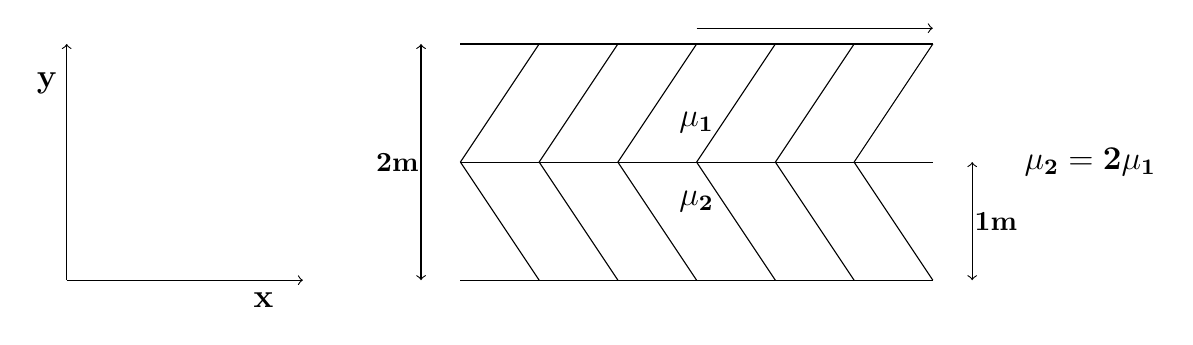
\begin{tikzpicture}
    \draw[->] (-5,0)--(-2,0);
    \draw[->] (-5,0)--(-5,3);
    \node at (-2.5,-0.25){\large $\mathbf{x}$};
    \node at (-5.25,2.5){\large $\mathbf{y}$};
    \draw (0,0) -- (6,0);
    \draw (0,3) -- (6,3);
    \draw (0,1.5) -- (6,1.5);
    \draw (0,1.5)--(1,3);
    \draw (1,1.5)--(2,3);
    \draw (2,1.5)--(3,3);
    \draw (3,1.5)--(4,3);
    \draw (4,1.5)--(5,3);
    \draw (5,1.5)--(6,3);
    \draw (0,1.5)--(1,0);
    \draw (1,1.5)--(2,0);
    \draw (2,1.5)--(3,0);
    \draw (3,1.5)--(4,0);
    \draw (4,1.5)--(5,0);
    \draw (5,1.5)--(6,0);
    \node[align = center] at (3,2){\large $\mathbf{\mu _1}$};
     \node[align = center] at (3,1){\large $\mathbf{\mu _2}$};
     \draw[<->] (-0.5,0)--(-0.5,3); 
     \node[align=center] at (-0.8,1.5){$\mathbf{2m}$};
     \draw[->] (3,3.2)--(6,3.2);
     \draw[<->] (6.5,1.5)--(6.5,0); 
     \node[align=center] at (6.8,0.75){$\mathbf{1m}$};
     \node at (8,1.5){\large $\mathbf{\mu _2 = 2\mu _1}$};
     
\end{tikzpicture}
}
\end{center}
